\documentclass{article}

\usepackage{geometry}
\usepackage{makecell}
\usepackage{array}
\usepackage{multicol}
\usepackage{float}
\usepackage{setspace}
\usepackage{changepage}
\usepackage{booktabs}
\usepackage{graphicx}
\usepackage{wrapfig}
\newcolumntype{?}{!{\vrule width 1pt}}
\renewcommand{\figurename}{}
\renewcommand{\thefigure}{}
\renewcommand\theadalign{tl}
\setstretch{1.40}
\setlength{\parindent}{0pt}
\graphicspath{ {./Images/} }

\geometry{top=12mm, left=3cm, right=4cm}
\title{22W 520.342 Englisch: Kultur-Schwerpunktthemen IV (Anglosphere)}
\author{Andreas Hofer}

\begin{document}
	\large
	\section*{Introduction}
	While the previous lecture focused on the US, this lecture is more focused on the Anglosphere. Several lecturers will talk about different English speaking cultures and how they relate to post-colonialism. Some examples are white history in Australia and how it relates to the Indigenous population of Australia, the history within the Carribbean as well as within Nigeria and South Africa. \\

	\section{Week 1: Pre-Post-Colonialism - 03.03.2022}

	Before you can talk about Post-Colonialism, you must first talk about Colonialism itself. Even though people in Europe are the descendants of colonial powers, exclusion would only server the opposite. \\
	Over time, the British Empire had colonies all over the world, at one point ruling over millions of people on all continents. \\
	After the British Empire, the USA gained global influence and are today holding over 580 military presences all over the world on all continents. \\
	But while these are powerful examples of colonialism, colonialism was not invented by the British having existed for at least 5000 years with the lower Nile region having colonised the upper Nile region. \\
	At the same time Colonialism is not the same as Imperialism, one of which establishes directly controlled footholds in foreign land, while the other aims ot influence foreign countries and cultures without directly owning them. \\
	Skipping to modern colonialism, often dubbed the "Age of Discovery", it mainly happened due to a wish to establish new travel and trade routes. By going through land, you often have to pay levies and taxes just to pass, increasing the prices. Sea, on the other hand, does not and would thus make goods either far cheaper or drastically increase profit. \\
	Over time these powers also started exerting a more direct control over territories in order to gain an economic advantage. This can be likened to early capitalism, with high costs and high risk, promising very high returns if they succeed. In South America this included Silver, Cotton as well as Cocoa and Coffee. This also led to the Transatlantic Slave Trade, as free labour decreases costs and thus increases profits. \\
	While this was a core factor, the establishment of new markets was also important. Most European countries with sea access founded their own "East India Trading Companies" in order to take part in the spice trade, later also becoming a political power and branching into many more ventures. \\
	As the Companies winded down and lost influence, new colonies were soon established in Africa, which was for a long time spared due to the need of slaves. \\
	In general colonialism is today heavily revised and is unlikely to represent reality at that time. \\
	Columbus especially is a prime example of altering the reality of his discoveries in order to impress his "investors" and secure further funding. He described the land as a "Garden of Eden" flowing with abundance. He also describes the inhabitants of the island he landed on merely as "Inhabitants", signifying that they aren't actually using it, making it thus justified to take it and make better use of it. \\
	\subsection{Civilisation and Natural Philosophy}
	At that time the Philosophy of Natural Law was laos wide spread, according to which it was not consciable to take a person's right away, including indigenous people. But at the same time they concluded that people who were not "civilised" enough gave up their god-given rights of personhood, justifying enslavement as they aren't really people. \\
	In general \textbf{Civilisation} was a term used to justify enslavement and exploitation as these people were simply less developed and required help. The poem of the "White Man's Burden" talks about the burden European white people have to bear as they have a responsibility to give civilisation to these savages and "elevate" them. \\
	As in US Schwerpunktthemen III, the example of Star Trek is used again with the same scene of the woman mistaking the crew for gods, as they were still in approximately the bronze age. His example uses her ancestors as a point in the past where they had less scientific knowledge than she does, just as the woman possesses less scientific knowledge than the crew does. This implies that all scientific advancement is linear and her path eventually all leads to the same goal. \\
	\subsection{Term Definition}
	\textbf{Post-Colonialism} is a term that seeks to understand the legacy of colonialism on former colonies. \textbf{Edward Said} famously said \textit{"Ideas, cultures, and histories cannot seriously be understood or studied without their force, or more precisely their configurations of power, also being studied."}. and is one of the most prominent people in post-colonialism. His book "Orientalism" from 1978 talks about the stereotypical view people in Europe have of the Middle East. The West came to define the East in a manner that was useful to themselves. The East was always portrayed as "mysterious" or "strange" and in general less civilised, while the West was better understood in general with more logic. \\
	Thus everything outside of the West was portrayed as the "Other", which provides an experience instead of being people with their own culture (Who would likely view the West a the "Other"). \\
	There are 4 steps of trying to identifiy post-colonialism:
	\begin{itemize}
		\item{The representation of non-europeans within cultural identity}
		\item{The role of language within a group of people and whether it legitimises or subverts the dominant power.}
		\item{Cultural Identity: Is it homogenised and stable or more hybrid and unstable?}
		\item{Cross-cultural interactions: See how non-Europeans are portrayed in contexts like these}
	\end{itemize}

	\section{Sun, Sheep and Spices? - 10.03.2022 - Martin Gabriel}

	The Carribbean was not part of the British empire but instead of the Spanish and Portuguese empires. \\
	The time of early colonialism is often called the \textit{Age of Discovery}, yet this is a rather controversial term as these lands were not 'discovered' per se but only found for Europe. \\
	The way historians focus on people is often not in accordance with reality, with \textbf{Magellan} for example not actually circumnavigating the world as he died on his way home. \\
	The question why colonialism happened is manifold and there are many different explanations:
	With the Age of Discovery, the nobility decreased in importance and cities gained importance. The amount of people venturing into the world also increased with Enlightenment as more people were keen on discovering the world. \\
	There is also a factor between the Christian powers and the Ottoman empire. This relation is connected to colonialism, as the powers in Europe thought the Ottoman Empire controlled the trading routes through the Arabic world and closed these routes. \\
	There were in fact other trading powers in Europe, like in Geneva or Genua who controlled the trade with Asia. This is why empires like Spain or Portugal were keen on opening new trade routes: In order to avoid having to go through Italy. \\
	Italy at that time was a very powerful player in the trading business, and was also very wealthy so these countries closely collaborated. \\
	Within the 8\textsuperscript{th} century only a small part in the northern Iberian peninsula remained Christian and from there the Christian reconquest happened. At that time many Muslims but also Jews lived there and many were very wealthy and powerful. \\
	Within the Iberian Peninsula the Christians and Muslims and Jews were very closely related culturally, which, when war happens can culminate in two things:
	\begin{itemize}
		\item{Either the conflict becomes less brutal as there is a perceived closeness and an unwillingness to savagely fight these closely related adversaries.}
		\item{But it can also culminate in an even more brutal war, as these similarities underline the differences even more.}
	\end{itemize}
	When the Christians reconquered the Iberian Peninsula, the Ottoman Empire was much more liberal in religious freedom, only really caring about people paying their taxes. \\
	While the reconquering happened, they also wanted to make some money while doing so. While this does not make the reconquering itself a less noble cause, there was a lot of brutality between the combatants. \\
	\subsection{Brazil - 15\textsuperscript{th} Century}
	When Europeans colonised Brazil, they only really inhabitated the coasts and didn't actually discover most of South America until a century later. The most important good taken from Brazil was the so called \textbf{Brazil Wood} which, when cut in half, yields a pulpy mass which can be worked into dye. This also caused the emergence of Amsterdam as it was there where the pulp was refined. \\
	The answer to why the Portuguese stayed around the coastline, is that around this colonialism the Portuguese only numbered about 1 million, with the \textbf{Tupi} people found on the coastline of Brazil having about the same number. They also stopped people from leaving the country as there weren't a lot of people in general. But with this small population the Portuguese were in no position to conquer Brazil. \\
	In Venezuela, the pearl trade emerged and this coast is still called pearl coast to this day. These pearls were brought back to Europe and caused a boom there. This boom was very short-lived though, as the natives used to harvest the pearls sustainably. When these pearls were harvested by the Europeans, they instead ripped them out of the seabed and didn't give them any time to recover in population and the pearls dissappeared. \\
	Throughout history many places that were colonised were exploited and destroyed long-term in order to generate short-term profit. \\
	At that time Seville was the most important port city, even though the city itself was not on the coast at all. It also had very close ties to Madrid. During that time Seville became the third largest city in Europe, only after Naples and London. It became one of the very first multicultural centres of Europe as it was very common to see people of all ethnicities there. \\
	When the first economic trade route was established is a subject of debate, ranging from the 12\textsuperscript{th} century to the 18\textsuperscript{th}. Martin Gabriel's opinion is form the 16\textsuperscript{th} century onwards, with woods being traded to Europe. In the 1650s Manila was founded as a trading hub. While the Philippines themselves were not important it posed as an important post to trade with China. \\
	China was for the longest time the most important trading partner, as it had as many inhabitants as all of Europe, was highly centralised and lusted for silver. \\
	The trade route consisted of traders bringing silver to Manila, where the Chinese traders trade it for mostly silk and porcellain. \\

	China was at that time a silver-based economy, as the tax-system at that time required it and China did not have a lot of silver. At that time silver in China was worth as much as 6 times of what it was worth in Europe. The tax system was later changed, which brought silver back to what it was worth in Europe. \\

	\begin{wrapfigure}{l}{0.55\textwidth}
	\hspace{-2cm}
	\includegraphics[scale=0.6]{Illegal_Trade.png}
	\caption{Legal (blue) and illegal (pink) trade routes}
	\end{wrapfigure}


	Since it was very profitable, there were also large amounts of illegal trade. As it doesn't show up in official documents it cannot be said how much trade was illegal. Statistics stemming from Buenos Aires estimated that during that time about 20\% of trade was legal and 80 \% of trade was illegal. 'Illegal' in this case means that traders did not sell their goods to the specified port, since it yielded more profit there. At that time Seville had a monopoly on South American trade, and any trade had to go through that city. In South America there were also 3 monopoly ports where trade was legal, and trades in all other ports were considered illegal. \\

	The main reason for these strict monopolies was that Atlantic trade was a very-high risk venture and the shortest time you would get any return on your investment was 1 year. To make sure that people have some kind of stable income, prices were fixed and you had to go to very specific ports. This made sense in an 18\textsuperscript{th} century context, while maybe not making sense from a 21\textsuperscript{st} century context.\\

	Many of the navigational instruments used by European explorers originated in Asia, so without Asia exploration and colonialism would not have been possible. \\
	In addition the first explorers to India and China used the long standing knowledge of West-African navigators to make their way to India and open up the trade with Europe. \\
	Languages were also influenced to a large extent within colonial settlements. In the Phillippines the Spanish established the trading post of Manila and soon started printing books, one of them called \textit{Doctrina christiana (The Bible) en letra y lengua china}, which covers the bible in Latin for the Chinese people. \\
	Within Mexico the indigenous people harvested the \textbf{Cochineal Beetle} to turn them into red dye. Shortly before that Constantinople fell, drying up the purple dye trade with Italy. Soon after the people declared not purple but red as the colour of cardinals. The indigenous people profitted greatly from this dye trade. When this boom happened, one pound of cochineal was worth 60 times that of sugar. During the Spanish Empire's lifespan, cochineal was the 2\textsubscript{nd} most important trade good after silver. \\
	The Spanish had a monopoly on cochineal, and was \textit{extremely} profitable. At some point the cochineal that a farmer in Mexico harvested was traded through Europe, to the Ottoman Empire, to India, to China to Japan, where the Shogun wore cochineal dyed capes. \\
	At the same time the \textbf{Transatlantic Slave Trade} also took off. At first the Dutch were the main suppliers of slaves in the Americas but over time the English took over. \\
	In Brazil the colonies mainly traded in diamonds and sugar. The planting and subsequent bruning of sugar plantations led to large amounts of deforestation in the east. \\
	Within India hundreds of small colonies appeared, with the French, Dutch, English and Danish having the majority of settlements. A settler usually had a life expectancy of 1 to 5 years, leading to many acting very short-term, as you had to make as much money as possible and then get out. \\
	Within South East Asia there existed several networks that colonies used to trade. The \textbf{Bay of Bengal Network} in India was the largest network. There were also other, smaller networks but most of them were controlled by the Chinese. They succeeded in keeping out European traders for quite a long time, while still trading in tea and exotic woods. \\
	The Chinese, while very influental, were not interested in taking new land, as China was already quite large. In order to exert influence, while not controlling the land itself, the Chinese accepted tribute from rulers all over Asia and even Africa, often taking a loss because they paid for the journey with the tribute not making up for it. But what it did do, was give the Chinese Emperor the impression that all of them saw the Emperor as the supreme ruler. \\
	The spice trade was also a very important trade. While the Portuguese never traded themselves, they still made a lot of money by controlling trade hubs and taking taxes from ships that passed through. This made sense because there just were not very many Portuguese. \\
	\textbf{Malacca} was the Portuguese capital in Asia. While they did live there, they only lived in their own enclaves, leaving the rest to the native population. The Dutch on the other hand, built the whole city and influenced the architecture in their colonies. \\
	Another very important spice was Nutmeg, only cultivated on the Banda Islands. There was such a demand in that spice that it was for some time worth 10 to 15 times that of gold. When the Dutch sought to break the monopoly from the Banda Islands, they cut down the trees there, killed the natives and started growing trees in other areas. \\
	\textbf{Japan} at that time was also an important trading power. Unlike other nations, the Japanese carefully chose who they traded with, refusing trade with most European nations. The Dutch were one of the only European people keeping trade relations with Japan. \\
	While you usually talk about nationalities when covering colonialism, nationality was of very little concern to the colonial empires themselves, and often very little of the [Insert Nationality] trading hubs had people of that nationality in them. \\
	The French too were a very enthusiastic colonial power. But unlike the Spanish who wanted money and spread religion, the French intended to bring civilisation to their colonies. While they sought to make a profit, they put culture and civilisation as their centrepiece. They divided their subjects into two groups:
	\begin{itemize}
		\item{Those that are 'worthy' and can be taught French culture and language and maybe someda acquired citizenship}
		\item{Those that were just 'not worth the effort' and were given an overseer to look after them but considered it unlikely that they would be able to be taught French culture or language}
	\end{itemize}
	The British Empire increased the size of its empire gradually over the 18\textsuperscript{th} and 19\textsuperscript{th} century. Their largest extent was after 1921, when they received several possessions after World War 1. In fact, in the 1930s there were far more colonies than in the 19\textsuperscript{th} century. At first the British Empire was even th elargest proponent of free trade, as they themselves did not have a large empire but as their empire grew and they got more land, they started staking out their claim, claiming all of 'their' land as theirs in order to keep out other powers. \\

	\section{Globalisation and the US - 17.03.2022}

	While we were handling colonialism last week, this week's focus is on US-American imperialism. With the end of the Cold War, the US saw themselves as the winners and spiritual successors to the British Empire. But there were ideas like that even before that. In 1901 W.T. Stead, a British journalist, talked about the 'The Americanisation of the World'. Francis Fukuyama went even further and declared Western ideals as the norm around the world, with the US having taken 'the baton' in the world. \\
	Connected with the cultural imperialism, this is usually also connected to \textbf{Globalisation}. \\
	Campbell and Kean define Globalisation as \textit{"The process of increasing connectivity, through which idead, capital, goods, services and people are transferred across national borders."}\\
	With the onset of globalisation people also call the planet to being 'flattened out' as to it having become less hierarchichal and more democratic and information being less restricted. But while things like the Arab Spring were anticipated to have a marked effect on the Arab world, this has yet to materialise. At the same time a common criticism of globalisation is that it leads to homogenisation as certain cultural values and franchises are normalised across the globe. \\
	During the Cold War the US considered themselves as the beacon of freedom and the USSR as the communist East with a few 'hot' wars happening via proxy in Korea or Vietnam. \\
	After World War 2 both the US and the USSR had very different goals with the world. While the US wanted willing customers for their goods in order to fuel the economic boom, through the Marshall Plan in Western Europe and parts of Asia, the USSR meanwhile was concerned about Germany reawakening once more (As had already happened twice now) and thus aimed to build a buffer zone between itself and Germany. Thus the Cold War starting position was born. \\
	Since the Marshall Plan was aimed to reinvigorate certain countries in Europe and Asia in order to keep them away from communism. During the Cold War American soldiers stationed throughout Europe actively encouraged the consumption of American media. There have also been \textbf{America Houses}, officially meant to promote de-Nazification, while also spreading American culture. They had an open library, where people could borrow American books, as well as offering English courses and holding American centered cultural events like concerts and readings. These houses were established all throughout Europe, from Norway to Italy, also using them as launching pads to spread American culture throughout Europe by, for example, library buses.
	Thus through Globalisation the US is bringing its product into other markets, replacing local brands due to their much depper pockets. This is one of the views held by the Frankfurt School. Due to
	When Coca-Cola wanted to establish itself in France, the newspaper 'Le Monde' decried this as the first step to deprivation. They considered the US as a nation of 'Fridges and Hamburgers'. American culture was even compared to Nazi Germany as they 'at least knew they were being invaded'.
	\begin{itemize}
		\item{Something called 'Coca-Cola Colonialism', later replaced by 'McDonaldisation', where American cultural companies like McDonalds and Coca-Cola spread throughout the world. Since these companies also bring American cultural values, this can lead to homogenisation as it replaces the unique culture of that area with the standardised items of the companies. Major tenets of this process are:
		\begin{itemize}
			\item{\textbf{Efficiency:} The optimal method of acomplishing a task. With Mcdonalds it is the fastest way of getting from being hungry to being full. Everything is geared towards efficiency.}
			\item{\textbf{Calculability:} Having quantifiable objectives. Instead of trying to deliver the best product (With taste being a very subjective and not quantifiable thing) to only focusing on sales. This means that instead of trying to deliver quality, trying to deliver as many products as possible. This has also led to the assumption that large sales equals good quality; The best product sells the most, which isn't necessarily the case.}
		 	\item{\textbf{Predictability:} Standardised and uniform services. Delivering the same product everywhere, means that people can know what to expect no matter where they are. This is the same with the employees in such places, having highly repetitive and predictable tasks.}
		 	\item{\textbf{Control:} Controlling every aspect of one's sale. Employees wear the same outfit, use the same greeting etc. This is achieved even better by machines, who by design always do a task the same way.}
		 \end{itemize}}	
	\end{itemize}

	\section{Gender and Sexuality in India - 24.03.2022}
	In India gender-diverse people are known as \textbf{Hijras} who are generally male-to-female transgender people. They are mainly performers for parties, as they are thought to bring auspicious blessings. They also perform on streets where they try to extract money from passerbys. They also often make money by selling good fortune on street lights. In India there are about 2 million Hijras, almost 20\% of the population of Austria. And yet they are marginalised by society. Todays Hijras often call themselves Transgender or TG in order to distance themselves from the historic term. \\
	Historically the single most important thing in a Hijra's life has been to achieve womanhood, through breast implants or acting 'feminine'. Despite wearing women's clothes and trying to act 'feminine', they do not see themselves as women, as they cannot bear children. \\
	Even though Hijras are considered 'demigods' and have spiritual powers, they are still discriminated against, as people are scared of being cursed. While there are reserved jobs for Hijras, they can often not be 'taken'. Even though people respect Hijras, people historically do not want a Hijra to be their teacher. \\
	Hijras often undergo chemical castration in order to achieve 'Nirvana' and receive the ability to curse and bless. In India there exist 7 Hijra communities. In order to be accepted into one, a Chela (Daughter) has to be adopted by a Guru (Teacher/Mother). A Guru has the life long responsibility to look after their Chelas monetarily and emotionally. They also share clothes to 'show their allegiance'. \\
	Some authors refute that this is not a system of kinship but a system of power that holds the communities together. \\
	Hijras often stand outside of cultural boundaries, and thus also often assume mannerisms that do not conform to the status quo of the area. This can include talking English instead of the local language variety. \\
	\textbf{Social Constructivism} is a theory about how people assume identities based on the circumstances and the world shapes how people form their identity. Hijras are often shaped by their interactions with society. Judith Butler asserts that gender is an act, something that someone does. \\
	As money was invested into social programs within India and Pakistan, NGOs were established through which these groups could be helped. Hijras often use themselves being marginalised in order to distribute condoms and other things to people. The reason why people in India these days use transgender instead of assuming the traditional identity, is that is generally seen as being part of the English-speaking middle class instead of being working class. As transgender is more widely known than Hijra, it makes it easier to raiser awareness and the fact that it is based in English also gives them a higher standing within society as compared to Hijras. Hijras often have negative stigmas associated with them, like not wanting to work or living in Hijra community. \\
	Within Hinduism, there are several gods who are in lesbian and gay relationships as well as gods which can change their sex at will. Before colonial times, Hijras generally enjoyed a favourable position within society. Religious texts also describe gender and sex diversity. Gender was considered not based on the soul, which they called \textit{atma}. Within Hinduism Shiva and Parvati together form the ultimate god, called \textbf{Ardhnareshwar}, which means 'Half man, half woman'. Within this context muslim rulers often considered Hijras valuable boons and offered them high positions as generals and advisers. It is estimated that in the past Islam was considerably more open to such concepts as they are today. After the British colonised India they criminalised non-conformation, which over time led to a change in attitudes of people. Some of these laws are:
	\begin{itemize}
		\item{Section 377 (1860) of the Indian Penal Code}
		\begin{itemize}
			\item{Acts against 'the order of nature' with any man woman or animal is imprisoned for life. Was based on the Buggery Act ofe 1533.}
		\end{itemize}
		\item{The Buggery Act (1533)}
		\begin{itemize}
			\item{Buggery is an 'unnatural sexual act', which included anal intercourse and bestiality. It was based on the notion that non-procreational sex to be against the will of God.}
		\end{itemize}
		\item{The Criminal Tribes Act (1871) of India}
		\begin{itemize}
			\item{Certain tribes including Hijras were considered of criminal nature restricting their occupation.}
		\end{itemize}
	\end{itemize}

	\section{From Cortés to Coca-Cola - 31.03.2022 - Martin Gabriel}

	The first settlement in the Americas was on the island of Hispañola, which is present Haiti/Dominican Republic. We often talk about national projects of colonisation with the Portuguese colonies in Brazil etc. but on Hispañola archaeological finds proved that there was not just one nation present. Finds on the island included Spanish cuenca tiles with clear Islamic influence. They also found thimbles (Fingerhüte) from Nuremberg, which was at that time the capital of textile production and (perhaps Afro-)American ceramics. Thus this island can be considered a multicultural hub in the Carribbean. \\
	At the same time \textbf{Hernan Cortés} is landing on the Mexican border with, mainly European but also some African, soldiers. One notable African soldier was \textbf{Juan Garrido}, who under Cortés led a life comparable to the Europeans, which he took by subjugating the Mexican people. \\
	From a language family perspective, native American languages show a relationship between the Aztecs and native American tribes. The Apache language specifically is a \textbf{Uto-Aztecan} language and thus more closely connected to the Aztec empire than other native American tribes like the Sioux or Cree. In general Uto-Aztecan languages were very widespread throughout northern and central America. \\
	Within the Aztec empire \textbf{Nahuatl} was the most commonly spoken language. After the Spanish conquest, language was used to drive colonialism; Nahuatl was banned and Spanish was promoted. At that time the language known as \textit{Spanish} was still called Castillian and originated around the area of Aragon. So in some sense, the Spaniards had just started formalising their own language, but were now trying to establish it in Mexico. To do that they started translating all of the books initially found in Nahuatl. The main purpose was, as always with the Spanish, to spread Catholicism. Some interesting points about these Spanish to Nahuatl translations is that they specifically left some words in Spanish. Some of them were \textit{Capitulo} (Chapter), \textit{Dio} (God) as well as other religious words. They feared that by translating these words they would undermine their own colonial efforts. Despite the Spanish colonial empire not having lasted very long, the Spaniards left a lasting impact in these areas. \\
	They had similar projects with the Maya empire further South, with the state and the church financing translations at a large scale. One notable difference in the Mayan empire was that the language that they called \textbf{Yucatec} (After the Yucata peninsula) was actually created by the Spaniards. The language that they initially called 'Reduced Mayan' was an amalgamation of several Mayan dialects from which they created Yucatec and used this to converse with their subjects. \\
	While the Spanish colonised central and southern America, the population remained polyphonic. A report from \textbf{Pedro Morales} in 1578, so several decades after colonisation, he talks about a procession where people sang in polyphony (4 voices), which was an introduction from the Spanish, as well as flutes and drums, which were common instruments at that time. The subject of the songs were saints that the Spanish prayed to, while they were conquering Mexico. Thus in a mixture of two cultures they sang in Nahutal, in a verse metre introduced by the Spanish, using traditional instruments about Catholic saints. This is one of the most commonly used examples of \textbf{Religious Idiosyncracy}. In Mexico you can often see Catholic baroque churches which could be built in Spain but there are no benches inside and instead people stand on rice and light various types of incense. \\
	Another example is the Cult of the Virgin of Guadalupe, which before the colonisation prayed to a fertility goddess replaced this goddess with the Virgin Mary spreading propaganda texts in order to establish Catholicism. The question whether these people actually pray to the Christian God (or the Virgin Mary) or their pre-colonial gods is not entirely clear. Often there were people who pretended to be Christian but secretly still kept cult figures and perhaps even imagined praying to pre-colonial gods while praying in a church. A common opinion at that time was that it was better to have a person be 90\% Christian than 0\%. Throughout the Spanish colonial empire's history they continously found people who were ostensibly baptised but still prayed to their pre-colonial gods. Even though they aggressively persecuted such cult followers, they never got rid of it completely. \\
	\subsection{Jamaica}

	Jamaica was the starting point of the English slave trade. When the English colonised Jamaica in 1655 it was of very high importance to the British Empire up until the late 18th century. At that time the colonies in North America were of little consideration to them. It was so important because of the large slave population and the labour-intense sugarcane plantations. The native population of Jamaica has long been wiped out by Epidemics and wars so they brought large amounts of slaves to the island. The sugar trade was at that time the most important trade good to the British Empire. While English people often moved to Jamaica, this was only to rule over the local population. With such a massive imbalance of races, at some point \textit{The Whitening} happened. This was purely an administrational change in order to increase the 'white' population by considering children of a black and a white person white (Mulattos). Despite what was commonly thought to be the status quo in America, almost everywhere else it was very normal for a black and a white person to have children and marry. This practice was suspended after a slave uprising in 1760. \\
	White Jamaicans, together with people on the Leeward Islands and Grenada, were the wealthiest citizens in America. The slaves were a large component of this wealth as it provided almost free labour. Jamaica was the unrivalled crown jewel of the British Empire which was only made possible through slaves. Another key factor in keeping the slave population in check were African supervisors, which were in turn given a better life. While this is often a fact that is glossed over, Africans were actively participating in the subjugation of other Africans. While one could say that they were 'traitors', one must consider that Africa is not a monolithic society and one ethnicity may like another ethnicity as much as they like their captors. Africans were also used to be in an environment where there are several 'players' and few felt some kind of racially motivated kinship with their peers but instead chose the side which guaranteed them the best outcome. \\
	With Jamaica having been so successful, it makes sense why the Brits seldom considered the 13 North American colonies as worthwhile. At that time Barbados alone was worth 10 times as much in exports. In fact to the British empire the independent United States were more important after they became their own country as compared to before. \\
	Over time a more hierarchical understanding of race came about. The common opinion was, that people from Africa cannot and will not be educated, it just wasn't possible. At the same time, as a more pragmatic reason, they kept any education from them in order to mitigate them rising up in any shape or form. \\
	When slavery was abolished in 1834 this school of thought could no longer feasibly exist and they had to try to educate their former slave population. But the former slave-holders were not too keen on considering their former slaves as 'equal', which is why they 'gave' them the English language as well as religion in order to keep them in check. Thus English became the language of prestige but only the 'correct' English. The English spoken by black people was by many at that time considered infantile - not fully formed. This was, even though it was intelligible, it was not considered English but Creole. Creole was a 'blending of various ingredients that originated in the Old World'. While we nowadays no longer consider languages as 'better' or 'worse' but just different, at that time there was a clear hierarchy and English, Spanish, French, German and Latin stood at the top and everything else was considered lesser. A similar viewpoint was that anything worthwhile created must have been created in Europe. This meant that it was readily accepted, that nothing worthwhile was ever created in Jamaica. \\ \\

	Another area of interest is the \textbf{Mosquito Coast} (Named after the Miskitu people, not the insect), which was an important source of tropical hardwoods to produce dye. Even though the coast was never officially considered a colony of British empire, it had large strategic importance, forming a triangle of sorts with Jamaica and Honduras. \\
	Belize was another colony within the British empire. Taken from the Spanish, it had a sizable population of people with Mayan ancestry. 62\% of the entire colony were Yucatan. After some time refugees from Mexico also fled to Belize changing the racial makeup even further. Just like with the Aztec empire, you can again find songs which show multiethnic properties. In Belize many songs are in English, but use Creole words with Spanish and English words mixed into it. The focal point of the local identity of the Creole people is often with the English people. In many parts of the Carribbean many people consider their heritage not in Africa but English woodcutters, a tradition that they, in their eyes, continued. \\

	\subsection{America 'civilising' the Caribbean}
	After the US had taken the Carribbean islands, the common opinion was that they had taken Cuba 'for the Cubans' who were unfortunately too inept to do it themselves. In general the US Army said that, while they were fighting 'for the Cubans' they had no love for them and would rather fight with the Spanish as at least those are European and not savages. \\
	For a bit the US considered the options for Cuba and whether it should become a colony, a protectorate or an independent state. Roosevelt said that independence for Cuba would be 'Anarchy for the savages'. Soon later in Haiti a similar question arose, with independence again being out of the question. At the same time though, companies like the \textit{United Fruit Company} started influencing the countries of central America. In the North people looked at the countries manipulated by these companies as weak as they would be too stupid to actually govern themselves anyway. \\
	Within Mexico in Teotitlán del Valle, which is very isolated from the West, terms of sexual-identity originating from popular American culture like \textit{gay, bisexual, homosexual} or \textit{lesbian} have started entering the vocabulary. But even Spanish words, like \textit{joto} and \textit{maricón} are starting to gain another sexual-identity related meaning meaning a passive homosexual man.

	\section{Post(?)colonial Caribbean and the UK - 07.04.2022}

	\subsection{THERE - in the Caribbean}
	By far the largest player in slave trade was Portugal. They are estimated to have bought 3.8 million slaves over time, while only 3.1 million actually arrived in America, with the rest having died on the journey. \\
	In the Caribbean there were a multitude of native tribes. The two most prominent were: The Caribs, also called Carribees, which survived long enough to have some form of influence on the area and the Arawaks, Natives of Jamaica, which is also what gave it its name from Xaymaca
	\begin{wrapfigure}{r}{0.5\textwidth}
	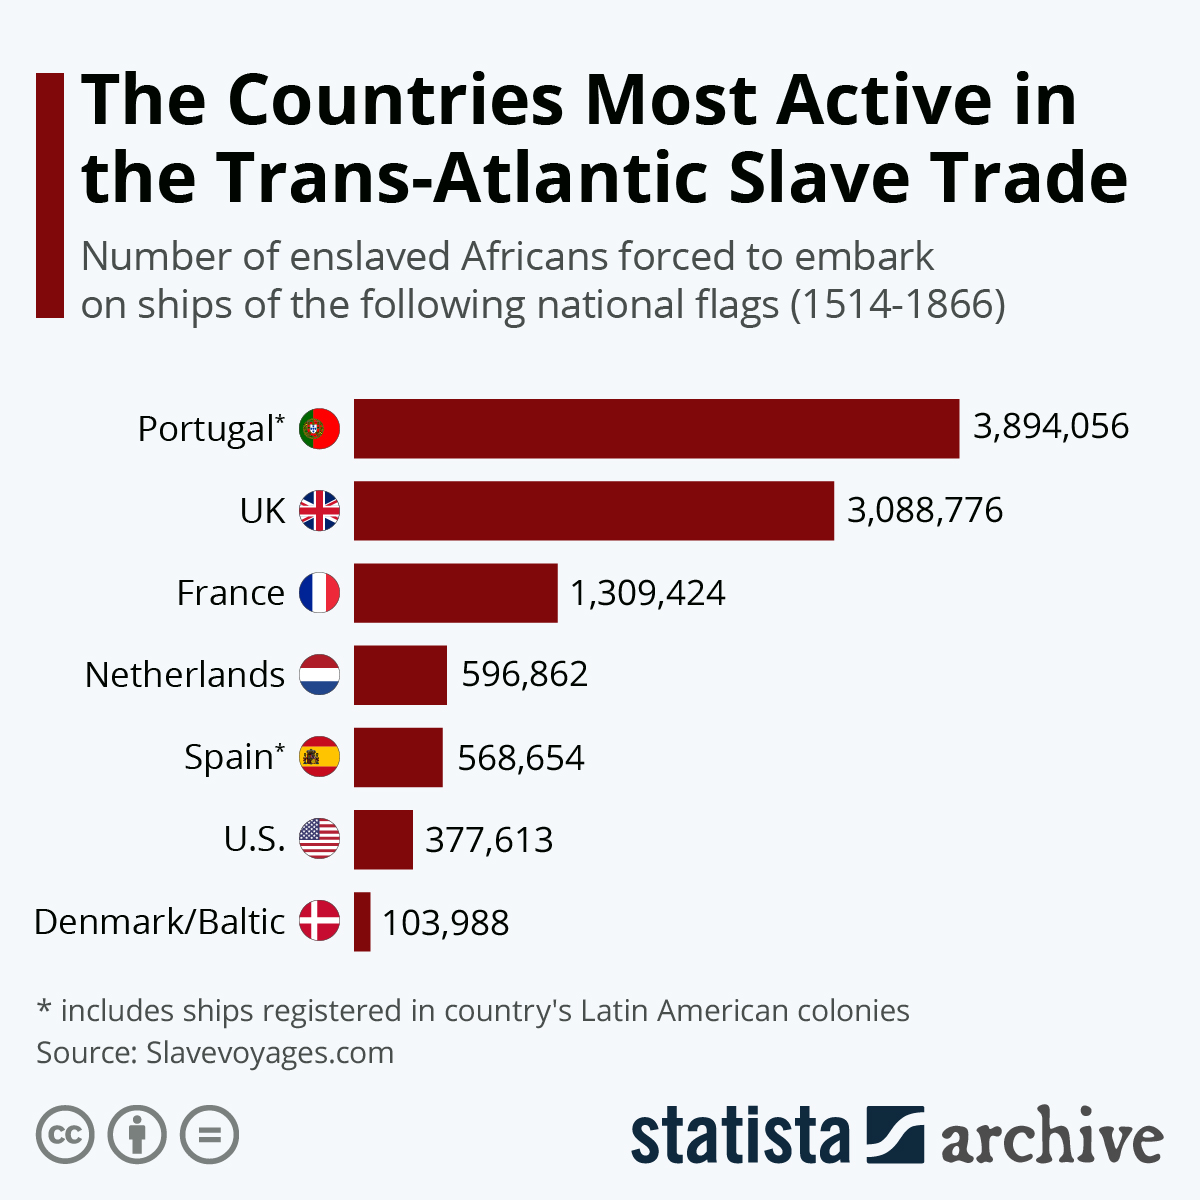
\includegraphics[scale=0.2]{Images/Slave_Trade.jpeg}
	\caption{Number of slaves purchased in Africa}
	\end{wrapfigure}
	Other than slavery, there was also indentured servitude, which is people who went into enough debt to having to work for their freedom. These were brought in after slavery ended, and labour costs were too high for the plantation owners. These were often brought from India, and the journey there was often the debt they had to repay. \\
	Even nowadays the influence from India can still be seen in the Caribbean. Curry is often used in Jamaican food and originally comes from India. Same with Ganja, which comes from Sanskrit. \\
	When these cultures clashed, a Creole language formed. Creloe languages are mixtures of many different languages (But often just two) which then form a new language in order ot facilitate interaction between the different people. But before a Creole forms, a pidgin is first created. A pidgin becomes a creole, the moment people grow up with a pidgin language. Despite this creole existing, English was still the more prestigious language, used in administration and taught in schools. \\
	In this context the distinction of \textit{Basilect}, \textit{Mesilect} and \textit{Acrolect} becomes relevant. 
	A Basilect is the dialect of a language, spoken mainly by people with less prestige. An Acrolect is the standardised version of a language which isn't necessarily spoken by anybody. The mesilect is thus the mixture of those two, and what most people speak on an everyday basis. In an Austrian context, Bavarian dialect is the Basilect, Austrian standard German is the acrolect and what people use is anything inbetween. \\
	\begin{wrapfigure}{l}{0.6\textwidth}
	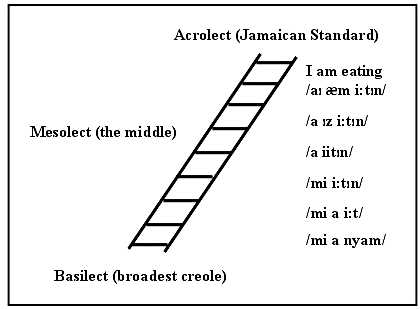
\includegraphics[scale=0.6]{Images/Jamaican.png}
	\caption{The flowing transition of Jamaican}
	\end{wrapfigure}
	In Jamaica, the language called \textbf{Patwa}, nowadays many people prefer calling it Jamaican, is such a Creole language. While in Jamaica English is still the administrative language, there are now efforts to formalise the writing and make Jamaican the administrative language. \\
	A comparison between Bob Marley and his son Damian Marley Jr. show the difference in social prestige that Patwa and English have/had then and now. When the BBC interviewed Bob Marley he still spoke Patwa during the interview, so he likely spoke very little English. Despite this, his songs were still almost always in English albeit with a very distinct accent. So he wrote his songs in English despite not being conversational in it, solely because Patwa as a language with low social prestige could not be used. One generation later with Damian Marley Jr. he very much knows English and is also able to speak it well (with a heavy accent) but chooses to write songs in Patwa, because Patwa is no longer of too low social prestige. Over time Patwa has increased in social prestige and is now in the process of replacing English as \textit{the} official language.

	\subsection{HERE - in the UK}
	Due to Britains colonial history, there has always been considerable migration to the UK. Slavery brought some Caribbeans to the UK, but it was very limited. During World War 2 they also allowed people to fight in the war but they had to go back after the war was over. In 1948 finally, there was a labour shortage, mainly due to losses during the war and they tried to replace those with Caribbeans coming to the UK. What the Mayflower was to the people in the US, the Windrush was to people coming from Jamaica. \\
	Due to this migration there were obviously frictions with people claiming that their jobs were being stolen. \\
	During the 1970s and 80s there was a period of recession and high unemployment, mainly due to the oil crisis of 1973, where the OPEC refused to sell oil to the UK. \\
	During that time youth unemployment was up to 4 times as high for Jamaican descendants than the general population. The Scarman report from 1981 came to the conclusion, that oppressive policing, unemployment and poverty had led to the riots. In addition so called \textbf{Sus Laws} were enacted to police black people without the requirement of suspicion. \\
	In 1985 over 20000 attacks on non-white Britons happened. 55 people were murdered every day; 2.2 people every hour. \\
	In 1998 the Macpherson report came to the conclusion that the police force was institutionally racist. \\
	\subsubsection{The Windrush Section}
	The so-called 'Home Office hostile environment policy' was enacted, where people who were in the UK illegally had to either go home or face jail. People who were affected had to prove that they were here legally. The landing cards, which are cards that people got when they left the ship to the UK, were destroyed by the government in 2010. Because of that, according to the Home Office 850 people were wrongfully detained and at least 20 were wrongfully deported. \\
	\subsection{Representation}
	Over time representation for Jamaicans increased. In Birmingham there is a Jamaican festival celebrating the independence of Jamaica. The TV-Show Desmond's from the 80s was one of the first to have a predominantly black cast. \\
	\subsection{Still There? - Legacy}
	So how is the UK still involved in Jamaica and other former colonies? \\
	They are still part of the Commonwealth of Nations. Another continued involvement is the \textbf{Judicial Committee of the Privy Council (JCPC)} which is the supreme court within the Commonwealth. In addition, 29\% of all lost tax revenue can be attributed to a former British colony or crown dependency. \\
	\subsubsection{Change?}
	Recently Barbados, Belize and Dominica and Guyana left the JCPC to join the Caribbean Court of Justice (CCJ).

	\section{More India - 28.04.2022}

	The first Indian people arrived around 50,000 years ago and settled around the Indus river. The river used to be called Indu, but the British could not pronounce it and called it Indus. The people that settled in the Indus river valley were known for their elaborate houses, which happened around 5000 years ago. \\
	Around 400 BC the \textbf{Caste System}, which decides a profession based on your father's profession, and punishes any mobilitxy harshly. At 1250 CE the Muslims arrived in India, of which there still are several buildings that date to this time. At some point they were replaced by the \textbf{Mogul} who ruled the country until they were replaced by the British. One building erected by the Moguls is the Taj Mahal, by Shah Jahan, who built it to mourn his wife. \\
	When the British arrived they stayed in the country until up to 1994. In 1857 they officially incorporated India as a Crown territory, making it a colony of the UK. They made themselves sound benevolent but the treaty was all but that. \\
	The TV-Show \textbf{Bridgerton}, has, according to Ankita, severely misrepresented Indian people. According to her many of the characters are little more than tokens. Some girls in the show look like they are from the south of the Country, but have north Indian Surnames and are upper caste. She also often refers to her father by a Tamil word, which is again in the south. \\
	Ankita wonders why, when they spent so much time on costumes and jewellery they couldn't also do some research on Indian cultures. She also asserts that by mixing all of these traits it gives Indians a hint of homogeny, while they are very much not. \\
	\subsection{British Colonial's History}
	When the British arrived in India it had a share of 23\% of the world trade. When they left again this was down to 4\%. \\
	This happened in part due to the British ruling India in their own interests. It is said, that when the British arrived in India, they were creating the finest Muslim clothes and had more than a quarter of the global finished clothing production. The British are said to have crushed the spinning wheels, broken the weaver's fingers and imposed heavy taxes. Over time India turned from a producer to one of the biggest importers of British goods. \textbf{Robert Clive}, often called "of India" aggressively ousted governors to get a monopoly on taxes, making 180,000 pounds over his time there, which amounts to 24 million pounds today. \\
	During WW1, 13 million Indians served for the UK, which constituted 1/6th of the forces. 65000 were killed, 4000 were missing and 20000 could not work again when they returned. It was the Indian people who had to bear the burden of reconstruction after the war had happened. \\
	There was a protest in Punjab to protest the living conditions. The governour ordered his soldiers to fire at the protesters, who fired until they ran out of ammunition killing 2000 people. \\
	When the UK left, they split India into Hindu and Muslim people, Pakistan and Bangladesh and India in the middle. Even though there were thousands of kilometres between the two parts, they were officially one country. Only later did they create their own country on the grounds of cultural differences. Estimated are that millions have been displaced due to this partition. It has also led to three wars between the two countries. \\
	It would be pointless to assert that the British Empire has to pay reparations. \\

	\section{Contemporary Society of India - 05.05.2022}
	\subsection{Colonial Legacy}
	Ankita has recently had a discussion with a friend of hers about the war in Ukraine. She mentions a picture published by the government about a woman who was being rushed to a hospital, where surgeries were performed to save the mother's and child's life, which she apparently dismissed as propaganda. Simultaneously she remembers her shedding tears at the movie "Once upon a time in Hollywood", where the cult of [[TODO ADD GUY Charlie Mansion?]] stops a woman from giving birth. Ankita assumes that the difference in the reactions stems from one having been a celebrity and the other one having been just a regular person. \\
	Recently there has been a paper published in the US about the opinion of people being largely formed by political party lines, due to the high partisanship of opinions. It challenges an often held belief that people who consume very biased news sources like Fox News by making people who generally watch news programs like that instead watch CNN for a month. After that time they were still firmly Republican but held slightly more progressive views, like being more open towards in-mail voting or no longer completely believing that Biden wants to defund all police. This implies that people's opnions can very much be changed although the study also mentions that after only 2 months almost all participants had stopped watching CNN once more in favour of Fox News among others. \\
	People in the US and the UK often assume themselves to have been the 'victors' of World War 2 and thus the good guys who can do no bad, making the approach to history a very black and white. But history has a history of 500 years before WW2 actually happened. But at the same time Ankita does not wish to discredit everything that the UK did in India as there were very much British people during the colonial times who helped the country as well as the colonial power itself having brought good things to the country. Instead it should require a more balanced approach to colonialism. According to her within the UK there are very few courses that directly handle the impact of colonialism like 13 million Indians serving in WW2 and 56000 dying during it, while having no stake in the war itself. \\
	\subsection{India Today}
	India is the world's largest democracy, with elections being held every 5 years. There are two houses, the upper house operates at a national level, while the lower house is on a more local level. Just like in Austria (and Germany) there is a Prime Minister (Which currently is Narendra Modi) and a president. While the Prime Minister is formally lower ranked than the president, the prime minister holds the real power while the president is supposed to be neutral and a figurehead of the nation. \\
	Nationalism used to not be negatively connotated. The only nationalism that existed within India for the longest time was the anti-colonialism movement. Only in recent years (About 10 years or two elections) has nationalism become associated with a sense of nation, while only allowing one way of life, namely the Hindu lifestyle. According to Ankita calling onself 'Liberal' has become negatively associated. This usually culminates in people considering people who don't support the current status quo as not being nationalistic and thus being anti-nationalist. \\
	The constitution states that 'India is Pared'. Pared is the traditional term for India used by Indian people. Within the constitution these two terms are considered interchangeable. But recently the government has been making a clear distinction between them. India is now being associated with the elite, and with speaking English and in general things that are against India as a country, while Pared is the name that the true Indians use. \\
	The 'Government of India Act', passed in 1934 by the British before they actually left, gave all people living in India and Bangaldesh the opportunity to become Indian citizens. This very specifically does not include a requirement of specific religions. But with a new law passed recently, called the 'Citizenship Amendment Act, that is meant to 'fasttrack citizenship to India', it specifies which religions can be considered for citizenship within this law. The list includes several religions including, Sikh, but excludes Islam. The justification for this is that nearby countries like Pakistan and Afghanistan are openly Islam nations and can thus not be persecuted. But other neighbouring countries like Myanmar are openly Buddhist and have notable Muslim minorities. India has for the longest time been an openly secular country (Secular in India means that the government embraces all religions instead of being detached from it like in Western countries), unlike Pakistan which from the very beginning called itself an Islamic nation, and only recently is now asserting that India is a country of Hindus. \\
	Thus India is now stating that they are openly rejecting Muslim refugees or are not in need of aid. There have been multiple protests in recent times but not by Muslims within India but rather people who refuse to accept this 'new order' of what it means to support your country. \\
	\subsubsection{Media in India}
	As a demonstration of the state of media within India Ankita showed us a clip of a news anchor and his guest shouting at each other about not standing during the national anthem as the guest, who is Muslim, did not want to and he considered it his choice. She prescribes this to the emergence of 24/7 news channels, as there has to always new things and people are starting to watch them for entertainment instead of getting information. \\
	\subsubsection{The Political Landscape}
	The current governmental party entered the political landscape with much fanfare of change, which according to her has not at all materialised. It is considered the richest political party in the world, while India itself is very much not a rich nation. The \textbf{Sangh Parivar}, a collective of nationalist groups, which includes the ruling party \textbf{Bharatiya Janata Party}, which Ankita chose to henceforth call 'The Family', considers a policy of \textbf{Hindutva}, which is different from Hinduism. According to them the country's history of secularism has negatively affected the lives of Hindus in India. An example given is the fact that despite polygamy being illegal in India, Muslims are exempt from this law as it is part of their religion. There is a very open goal of abolishing any special rights minorities within India might enjoy. \\
	Another justification of this policy is the site of a Mosque, where according to legend a Hindu temple once stood, which is the birthplace of an important Hindu God. \\
	There are widely considered stereotypes about Muslims, that they are dirty, or that they spread diseases and that they 'steal good Hindu girls'. During rallies it can often be heard advising people to protect their children from Muslim boys or they will take them and convert them to Islam and multiply as Muslims have many Muslim children. \\
	Just like a good right-wing party they create a narrative of an impending threat to the Hindu lifestyle, which the Family will protect them from. \\
	Ankita considers another factor about people 'becoming more stupid'. Apparently WhatsApp messages proliferated about questionable cures to Covid or cancer or other illnesses. People consider information found on the internet to be verified if it confirms their own view (I remember confirmation bias).
	\subsubsection{Covid}
	As a bonus she also spoke of the Covid wave. It reached India very late, when it had already swept over Europe and North America. The president turned up and said that the country is going into a lockdown. This happened 2 hours later. Many of the seasonal workers, which were far away from their homes, were suddenly out of work. As a consequence many families started walking home, which led to many deaths and the further spread of Covid across the country. One incident was that people thought that trains were not operating and thus slept on the railway during their journey home. Unfortunately one random train engine, without any cargo or passengers, came across this track and killed 17 people in the process. Another incident was that the prime minister suddenly announced, that 500 and 1000 Rupee bank notes (Equivalent to 6 and 13 €) were no longer valid, which led to thousands of people rushing to ATMs to exchange their money. This led to several deaths due to heat stroke from standing in the sun for too long. The reason given was the hope of transforming India into a cashless society, to curb the spread of the virus as well as stopping funding for terrorists, as they apparently cannot use debit cards.
	
	 


	
	
	
























	
\end{document}